\begin{figure}[t]

\captionsetup[subfigure]{aboveskip=-7pt,belowskip=-1pt}

\centering

\newcommand{\myuniquefoursize}{0.32\columnwidth}

\begin{subfigure}[b]{\myuniquefoursize}
\centering
\cfbox{box-gray}{
\resizebox{!}{\textwidth}{
% \tikzsetnextfilename{model3}
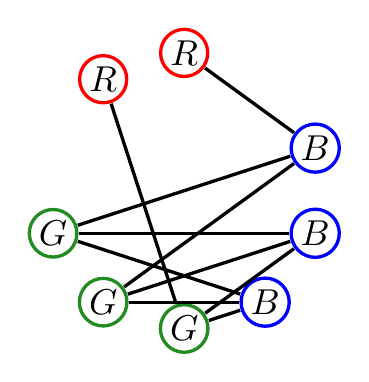
\begin{tikzpicture}[
mynode/.style={draw, circle, very thick, inner sep=1pt, scale=1.3},
myline/.style={draw, very thick},
]
\pgfmathsetmacro{\n}{10};
\pgfmathsetmacro{\r}{1.75};

\node[mynode,draw=red] (1) at (0*360/\n + 90: \r cm)  {$\xcolor{R}$};
\node[mynode,draw=red] (2) at (1*360/\n + 90: \r cm)  {$\xcolor{R}$};
\node[mynode,draw=none] (3) at (2*360/\n + 90: \r cm)  {$\phantom{G}$};
\node[mynode,draw=ForestGreen] (4) at (3*360/\n + 90: \r cm)  {$\xcolor{G}$};
\node[mynode,draw=ForestGreen] (5) at (4*360/\n + 90: \r cm)  {$\xcolor{G}$};
\node[mynode,draw=ForestGreen] (6) at (5*360/\n + 90: \r cm)  {$\xcolor{G}$};
\node[mynode,draw=blue] (7) at (6*360/\n + 90: \r cm)  {$\xcolor{B}$};
\node[mynode,draw=blue] (8) at (7*360/\n + 90: \r cm)  {$\xcolor{B}$};
\node[mynode,draw=blue] (9) at (8*360/\n + 90: \r cm)  {$\xcolor{B}$};
\node[mynode,draw=none] (10) at (9*360/\n + 90: \r cm)  {$\phantom{B}$};

\draw [myline] (9) -- (1);
\draw [myline] (6) -- (2);
\draw [myline] (7) -- (4);
\draw [myline] (8) -- (4);
\draw [myline] (9) -- (4);
\draw [myline] (7) -- (5);
\draw [myline] (8) -- (5);
\draw [myline] (9) -- (5);
\draw [myline] (7) -- (6);
\draw [myline] (8) -- (6);

\end{tikzpicture}
}
}
\caption{\mypm{}~{\scriptsize 1307670379328}}
\end{subfigure}
%
%
%
\begin{subfigure}[b]{\myuniquefoursize}
\centering
\cfbox{box-gray}{
\resizebox{!}{\textwidth}{
% \tikzsetnextfilename{model3}
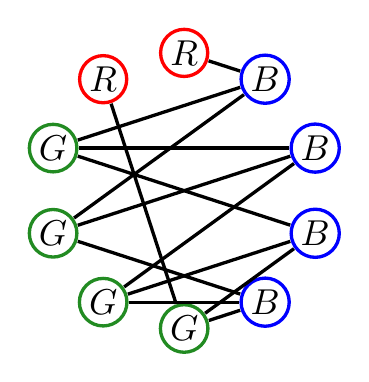
\begin{tikzpicture}[
mynode/.style={draw, circle, very thick, inner sep=1pt, scale=1.3},
myline/.style={draw, very thick},
]
\pgfmathsetmacro{\n}{10};
\pgfmathsetmacro{\r}{1.75};

\node[mynode,draw=red] (1) at (0*360/\n + 90: \r cm)  {$\xcolor{R}$};
\node[mynode,draw=red] (2) at (1*360/\n + 90: \r cm)  {$\xcolor{R}$};
\node[mynode,draw=ForestGreen] (3) at (2*360/\n + 90: \r cm)  {$\xcolor{G}$};
\node[mynode,draw=ForestGreen] (4) at (3*360/\n + 90: \r cm)  {$\xcolor{G}$};
\node[mynode,draw=ForestGreen] (5) at (4*360/\n + 90: \r cm)  {$\xcolor{G}$};
\node[mynode,draw=ForestGreen] (6) at (5*360/\n + 90: \r cm)  {$\xcolor{G}$};
\node[mynode,draw=blue] (7) at (6*360/\n + 90: \r cm)  {$\xcolor{B}$};
\node[mynode,draw=blue] (8) at (7*360/\n + 90: \r cm)  {$\xcolor{B}$};
\node[mynode,draw=blue] (9) at (8*360/\n + 90: \r cm)  {$\xcolor{B}$};
\node[mynode,draw=blue] (10) at (9*360/\n + 90: \r cm)  {$\xcolor{B}$};

\draw [myline] (10) -- (1);
\draw [myline] (6) -- (2);
\draw [myline] (8) -- (3);
\draw [myline] (9) -- (3);
\draw [myline] (10) -- (3);
\draw [myline] (7) -- (4);
\draw [myline] (9) -- (4);
\draw [myline] (10) -- (4);
\draw [myline] (7) -- (5);
\draw [myline] (8) -- (5);
\draw [myline] (9) -- (5);
\draw [myline] (7) -- (6);
\draw [myline] (8) -- (6);

\end{tikzpicture}
}
}
\caption{\mypm{}~{\scriptsize 1608847915988}}
\end{subfigure}
%
%
%
\begin{subfigure}[b]{\myuniquefoursize}
\centering
\cfbox{box-gray}{
\resizebox{!}{\textwidth}{
% \tikzsetnextfilename{model3}
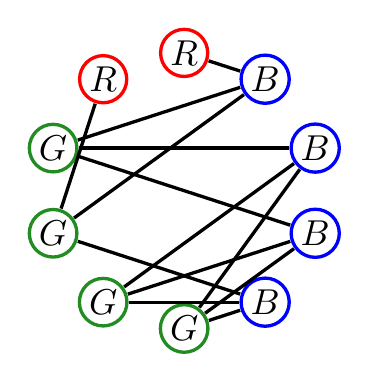
\begin{tikzpicture}[
mynode/.style={draw, circle, very thick, inner sep=1pt, scale=1.3},
myline/.style={draw, very thick},
]
\pgfmathsetmacro{\n}{10};
\pgfmathsetmacro{\r}{1.75};

\node[mynode,draw=red] (1) at (0*360/\n + 90: \r cm)  {$\xcolor{R}$};
\node[mynode,draw=red] (2) at (1*360/\n + 90: \r cm)  {$\xcolor{R}$};
\node[mynode,draw=ForestGreen] (3) at (2*360/\n + 90: \r cm)  {$\xcolor{G}$};
\node[mynode,draw=ForestGreen] (4) at (3*360/\n + 90: \r cm)  {$\xcolor{G}$};
\node[mynode,draw=ForestGreen] (5) at (4*360/\n + 90: \r cm)  {$\xcolor{G}$};
\node[mynode,draw=ForestGreen] (6) at (5*360/\n + 90: \r cm)  {$\xcolor{G}$};
\node[mynode,draw=blue] (7) at (6*360/\n + 90: \r cm)  {$\xcolor{B}$};
\node[mynode,draw=blue] (8) at (7*360/\n + 90: \r cm)  {$\xcolor{B}$};
\node[mynode,draw=blue] (9) at (8*360/\n + 90: \r cm)  {$\xcolor{B}$};
\node[mynode,draw=blue] (10) at (9*360/\n + 90: \r cm)  {$\xcolor{B}$};

\draw [myline] (10) -- (1);
\draw [myline] (4) -- (2);
\draw [myline] (8) -- (3);
\draw [myline] (9) -- (3);
\draw [myline] (10) -- (3);
\draw [myline] (7) -- (4);
\draw [myline] (10) -- (4);
\draw [myline] (7) -- (5);
\draw [myline] (8) -- (5);
\draw [myline] (9) -- (5);
\draw [myline] (7) -- (6);
\draw [myline] (8) -- (6);
\draw [myline] (9) -- (6);

\end{tikzpicture}
}
}
\caption{\mypm{}~{\scriptsize 1925189492487}}
\end{subfigure}
%
%
%

\caption{All 3 unique graphs for the NSCs in \nameref{sec:example3}.\label{fig:unique4}}

\end{figure}